%%%%%%%%%%%%%%%%%%%%%%%%%%%%%%%%%%%%%%%%%
% Programming/Coding Assignment
% LaTeX Template
%
% This template has been downloaded from:
% http://www.latextemplates.com
%
% Original author:
% Ted Pavlic (http://www.tedpavlic.com)
%
% Note:
% The \lipsum[#] commands throughout this template generate dummy text
% to fill the template out. These commands should all be removed when 
% writing assignment content.
%
% This template uses a Perl script as an example snippet of code, most other
% languages are also usable. Configure them in the "CODE INCLUSION 
% CONFIGURATION" section.
%
%%%%%%%%%%%%%%%%%%%%%%%%%%%%%%%%%%%%%%%%%

%----------------------------------------------------------------------------------------
%	PACKAGES AND OTHER DOCUMENT CONFIGURATIONS
%----------------------------------------------------------------------------------------

\documentclass{article}

\usepackage{fancyhdr} % Required for custom headers
\usepackage{lastpage} % Required to determine the last page for the footer
\usepackage{extramarks} % Required for headers and footers
\usepackage[usenames,dvipsnames]{color} % Required for custom colors
\usepackage{graphicx} % Required to insert images
\usepackage{listings} % Required for insertion of code
\usepackage{courier} % Required for the courier font
\usepackage{textcomp} % Required for the courier font
\usepackage{float} % for positioning pictures
\usepackage{lipsum} % Used for inserting dummy 'Lorem ipsum' text into the template
\usepackage{bbm} % indicator function

% Margins
\topmargin=-0.45in
\evensidemargin=0in
\oddsidemargin=0in
\textwidth=6.5in
\textheight=9.0in
\headsep=0.25in

\linespread{1.1} % Line spacing

% Set up the header and footer
\pagestyle{fancy}
\chead{\hmwkClass\ : \hmwkTitle} % Top center head
\rhead{\firstxmark} % Top right header
\lfoot{\lastxmark} % Bottom left footer
\cfoot{} % Bottom center footer
\rfoot{Page\ \thepage\ of\ \protect\pageref{LastPage}} % Bottom right footer
\renewcommand\headrulewidth{0.4pt} % Size of the header rule
\renewcommand\footrulewidth{0.4pt} % Size of the footer rule

\setlength\parindent{0pt} % Removes all indentation from paragraphs


%----------------------------------------------------------------------------------------
%	NAME AND CLASS SECTION
%----------------------------------------------------------------------------------------

\newcommand{\hmwkTitle}{Programming Assignment\ \#4} % Assignment title
\newcommand{\hmwkDueDate}{Monday,\ December\ 1,\ 2014} % Due date
\newcommand{\hmwkClass}{CS553\ } % Course/class
\newcommand{\hmwkClassTime}{} % Class/lecture time
\newcommand{\hmwkClassInstructor}{Ioan Raicu} % Teacher/lecturer
\newcommand{\hmwkAuthorName}{Thomas Dubucq / Tony Forlini / Virgile Landeiro Dos Reis} % Your name

%----------------------------------------------------------------------------------------
%	TITLE PAGE
%----------------------------------------------------------------------------------------

\title{
\vspace{2in}
\textmd{\textbf{\hmwkClass:\ \hmwkTitle}}\\
\normalsize\vspace{0.1in}\small{Due\ on\ \hmwkDueDate}\\
\vspace{0.1in}\large{\textit{\hmwkClassInstructor\ \hmwkClassTime}}
\vspace{3in}
}

\author{\textbf{\hmwkAuthorName}}
\date{} % Insert date here if you want it to appear below your name

%----------------------------------------------------------------------------------------

\begin{document}

\maketitle

%----------------------------------------------------------------------------------------
%	TABLE OF CONTENTS
%----------------------------------------------------------------------------------------

%\setcounter{tocdepth}{1} % Uncomment this line if you don't want subsections listed in the ToC

\newpage
\tableofcontents
\newpage

%----------------------------------------------------------------------------------------
%	Introduction
%----------------------------------------------------------------------------------------

% To have just one problem per page, simply put a \clearpage after each problem

\section{Introduction}

The goal of this programming assignment is to enable us to gain experience with Amazon Web Services such as EC2 Cloud, SQS queuing service and DynamoDB. The primary aim of this assignment is to implement a dynamic task provisioner. Our framework is divided into three parts: a client which submits tasks, the front end scheduler which handles the jobs distribution and scheduling and eventually the workers which runs the tasks either locally or remotely.\\ 

We are to use both SQS and DynamoDB in order to handle the replication of jobs in the scheduler part of this project. Finally we will measure the performance of our framework for throughput and efficiency according to the number of workers and the duration of the sleep tasks of the workers. Our project is implemented using Java language and helped with the AWS APIs. It uses Apache Ant to help the compilation process.

\begin{figure}[H]
\centering
\begin{tabular}{cc}
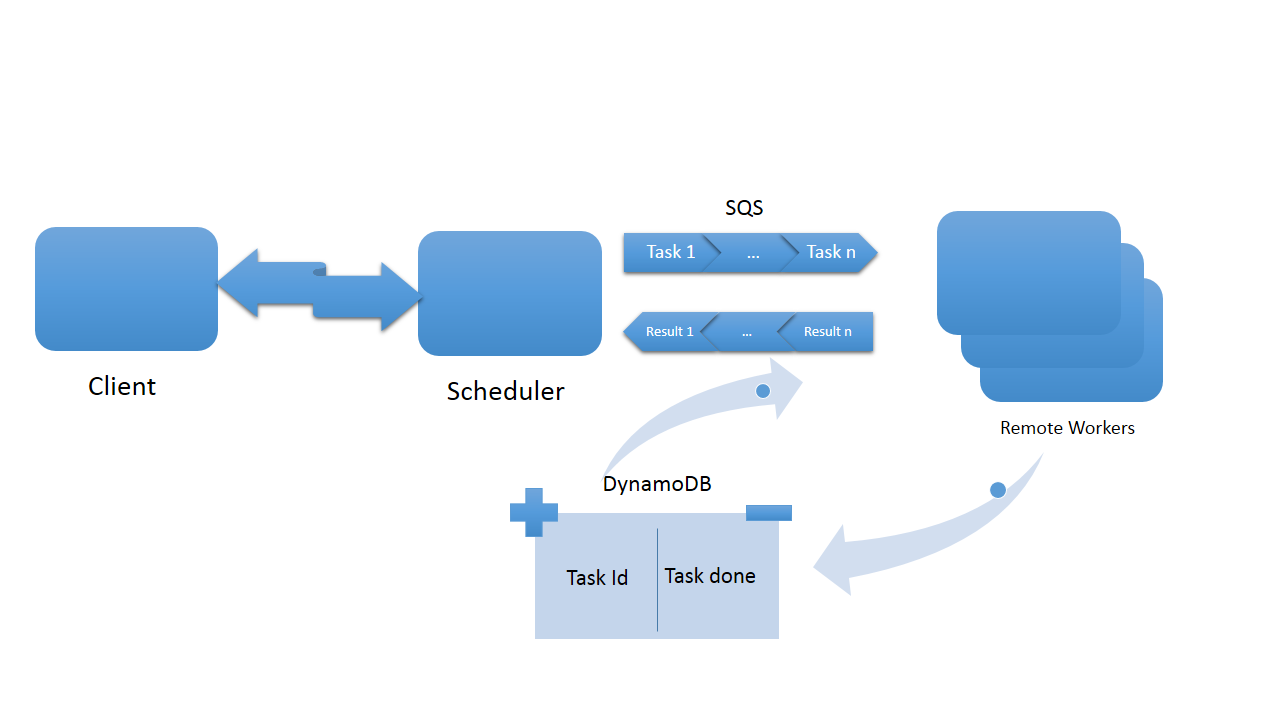
\includegraphics[width=0.8\textwidth]{Presentation1.png}
\end{tabular}

\caption{Framework layout}

\end{figure}

\section{The Task Execution Framework}
\subsection{The Client}
We implemented the client in the Client class. The client takes in argument the IP address/Port number of the front-end server used for scheduling using the following line command format:

\\
\verb+client -s <IP_ADDRESS:PORT> -w <WORKLOAD_FILE>+
\\

The workload file is a file containing the different tasks that the workers have to launch. In our case these tasks are sleep tasks followed by the duration of the sleep.\\

We used Java sockets in order to make the client and the scheduler communicate. First we parse the command line arguments to create the socket.\\

We also created a Task object which contains attributes such as the Id of the task, the arguments which are the task nature (here sleep) and the argument (here duration), a boolean which indicates if the task has been completed and finally the result of the task (0 if worked, else 1). Thus we can parse the workload file into a list of tasks which is sent to the scheduler. Moreover, the Task class implements the Runnable Java interface so we can run it easily in the workers. The \verb+run+ method just uses the task nature and arguments described previously to run the corresponding job.\\

The client also polls the scheduler every 100 milliseconds in order to keep track of the result of the jobs which has been submited from the workload file.

\subsection{The Front-End Scheduler}
The front end scheduler is implemented in the Scheduler class. 
The scheduler takes a command line argument which is the port number used to communicate with the client and an argument which sets the workers on "local" or "remote". If we use local workers, we have to define the number of local workers which corresponds to the numbers of threads which will run the sleep jobs. If we run the remote workers, we have to choices:
\begin{enumerate}
	\item by giving a number of remote workers in the command line, the scheduler will use static providing;
	\item otherwise, the scheduler will use dynamic providing.
\end{enumerate}

We first used a Java socket to retrieve the tasks from the client. \\

Then we put those tasks in a blocking queue in order to be able to run the threads for the local workers. We also implemented a threadpool which contains and runs the number of threads provided by the client to execute the tasks.\\

In the remote worker case, we first create a SQS queue that we fill with the jobs from the workload. We also create a DynamoDB table in order to help workers to avoid to run a taks twice because of the replication of data inherent to the Amazon SQS queuing service.\\

In that database we store the task Id and an integer initialized at zero and which is set at 1 by a worker when he pulls the task from SQS. If a worker finds a task which is already set to 1, the worker gives up the task and pulls another one from the queue.\\

Finally the scheduler pulls the results from the workers and sends it to the client through the socket

\subsection{Local Back-End Workers}
The local back end workers have been implemented within the WorkerThread class. These workers take in input the blocking queue filled with the tasks from the workload, and fills the result queue after running the corresponding sleep tasks.\\ 

These worker are used in the threadpool in the local back-end which is in the scheduler. At the end of the queue, "kill pills" are added - one for each thread launched - so that when all jobs are completed, threads will one after the other pull a kill pill from the queue, and will stop themselves.\\

As we previously said, the number of threads to run the tasks is set from the scheduler command line and used in the threadpool.

\subsection{Remote Back-End Workers}

We implemented the remote back-end workers in the SQSWorker class. The workers first pull a message from the SQS queue corresponding to a task. Then they look into the DynamDB table implemented in the TaskTable class:\\

if the task\_done field is set on 0 they set it on 1 and they run the task, otherwise they give up the task and pull another one from the SQS queue. When a worker pulls a message from the queue, it deletes it right after to avoid replication.\\

All the EC2 instances which are actually the remote workers run automatically the SQSWorker main method: this is done by using the user-data that can be transmitted to a launching instance and allows us to run a shell script on the instance right after it launched. These EC2 instances are working while they don't reach the idleness threshold which is set up to 30 by default. We are to speak about the dynamic provisionning of the workers in a further section.

\subsection{Duplicate Tasks}
This section just sums up what we already explained about the replication of tasks inherent to Amazon SQS service. In fact these queues are replicated for resilience purpose across diferent locations.\\ 

When a worker pulls a task and then removes the message from the queue, there is a chance that another worker has the time to pull a replicated message from the queue before it is actually removed. \\

That is why we need the use of a DynamoDB database to keep track of the status of each task and make sure that each task is processed only once in order to make our framework scalable.\\

\subsection{Dynamic Provisioning of Workers}
The dynamic provisioning of workers is aimed at increasing the ammount of instances working depending on the workload size. If the queue is growing over a certain amount of time, new workers will be created. On the contrary, we already explained that idle workers shut down themselves after reaching the idleness threshold if there is too much workers for a given workload.\\

We implemented the dynamic provisioning of the workers within the DynamicWorkers class. This object periodically watches the size of the SQS queue and runs new EC2 instances when the size of the queue increased from the last poll. The polling period is a parameter given at the creation of a instance of the DynamicWorkers class.\\


\section{Performance Evaluation}

In this section we will perform some measures which are respectively task throughput and efficiency based on the same model as the Falkon paper provided with the assignment. We first study the behavior of local workers which are run on the front end scheduler. Then we will take a look at the remote workers performance.\\


For the local workers we want to determine the maximum throughput which means that our tasks have to be as small as possible to evaluate the statically provisioned system that we implemented. As a consequence we implemented a script to provide a workload file containing 10K one-second sleep tasks. By running such fast jobs, we can observe the behavior of the workers while sharing the tasks which should be as efficient as possible to make the system scalable.\\

We also want to make the number of local workers vary to study if it is preferable to use a great number of worker to make the system scalable. Our measure is to plot the number of tasks processed divided by the total time from submission of the first task to the completion of the last task in the diagram below:


\subsection{Throughput and Efficiency}
\begin{figure}[H]
\centering
\begin{tabular}{cc}
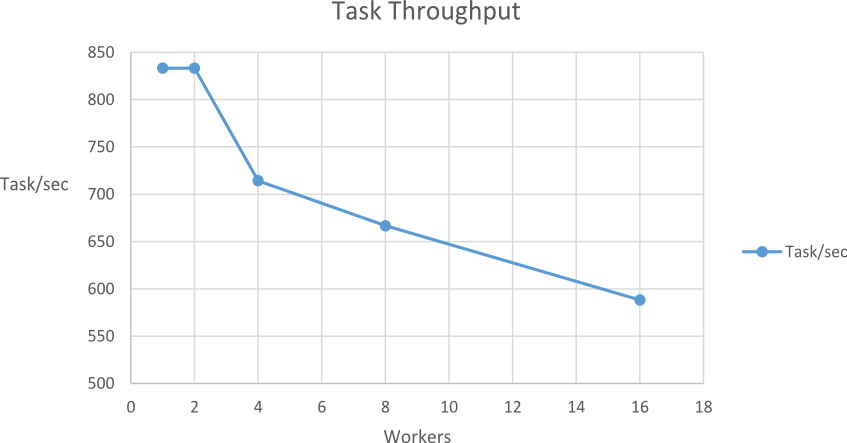
\includegraphics[width=0.9\textwidth]{Throughput.png}
\end{tabular}
\caption{Throughput}
\end{figure}

We observe that the throughput is decreasing when we increase the number of local workers. We can explain that observation by the fact that the time to set up the threadpool and to merge the threads involves overhead, since the tasks are "empty". Thus the more workers, the more overhead which leads to a poorer throughput. This observation might have been different with real tasks that requires more computation or more executing time.\\

Then we also want to make the tasks vary to make the study more accurate. Thus we will be able to measure efficiency which is the ratio of the theoritical execution time over the measured time. Then we have 25 different experiences to run. We want to make the workload fairly spread across the workers.\\ 

The number of tasks should be 80 per worker for 1 second tasks, 40 per worker for 2 seconds tasks, 20 per worker for 4 seconds tasks and 10 per worker for 8 seconds tasks. As we increase the number of workers, the aggregate number of tasks will also increase to keep a theoritical process time to 80 seconds.

\begin{figure}[H]
\centering
\begin{tabular}{cc}
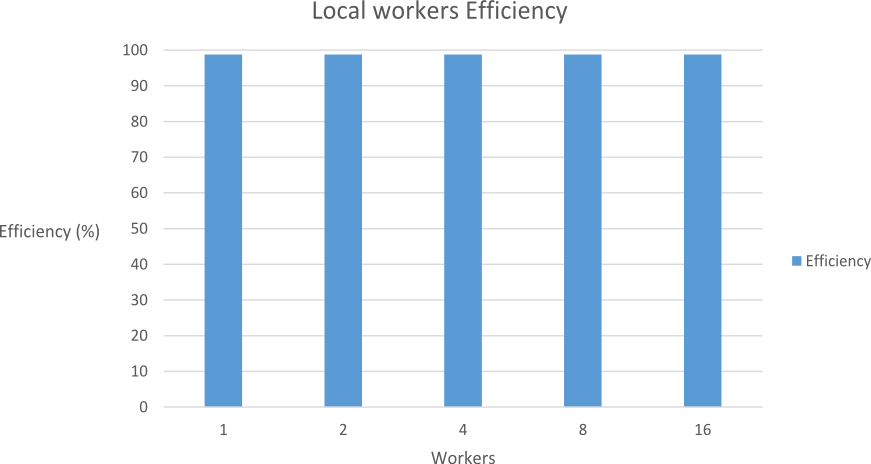
\includegraphics[width=0.9\textwidth]{local_workers.png}
\end{tabular}
\caption{Efficiency}
\end{figure}

We observe that the efficiency remains the same whether the task nature is varying or the number of workers is varying. Since we are using the local workers to run equivalent  workloads according to the number of workers, it seems logic that the execution time is roughly the same for each distribution. The difference of execution time is in the order of milliseconds, thus the efficiency remains almost constant for each workload.\\

Now we are to study the behavior of the remote workers while running the same workload and varying the amount of workers. Contrary to the local workers, the more workers we launch the more throughput we should have since the aim of such distributed system is to efficiently distribute the jobs in order to be able to scale.

\begin{figure}[H]
\centering
\begin{tabular}{cc}
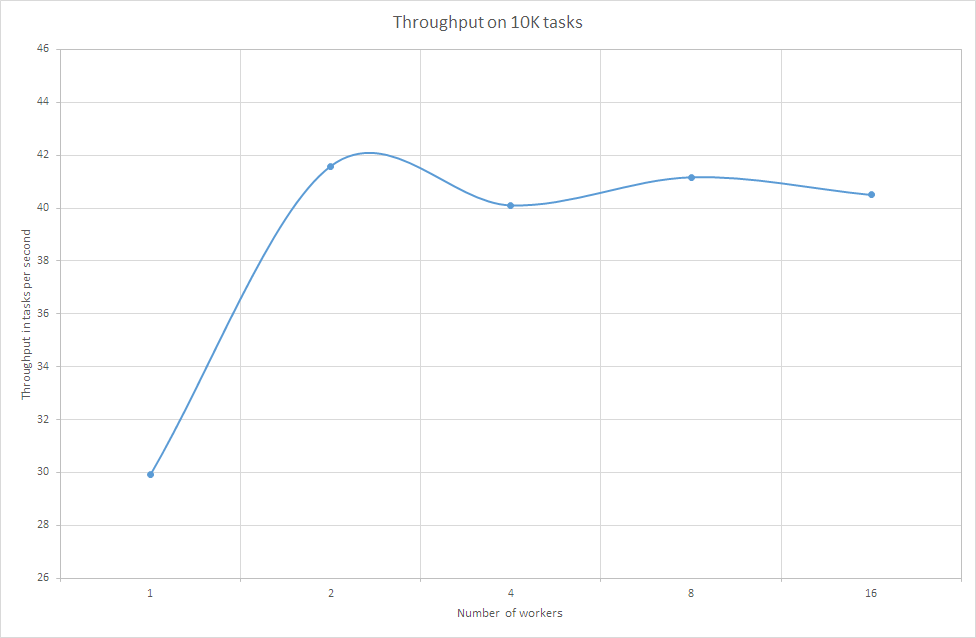
\includegraphics[width=10cm, height=6cm]{throughput_remote_workers.png}
\end{tabular}
\caption{Remote workers throughput}
\end{figure}

Compared with the local workers, the throughput is way slower. This is caused by the network additional delay that remote workers face compared to local workers that are using exclusively local memory. Nevertheless, we observe an increase of the throughput with the number of workers which eventually converges towards a threshold of 41 task per second.\\

Now we want to compare the efficiency of the remote workers with the local workers' one following the same experiences as previously:
\begin{figure}[H]
\centering
\begin{tabular}{cc}
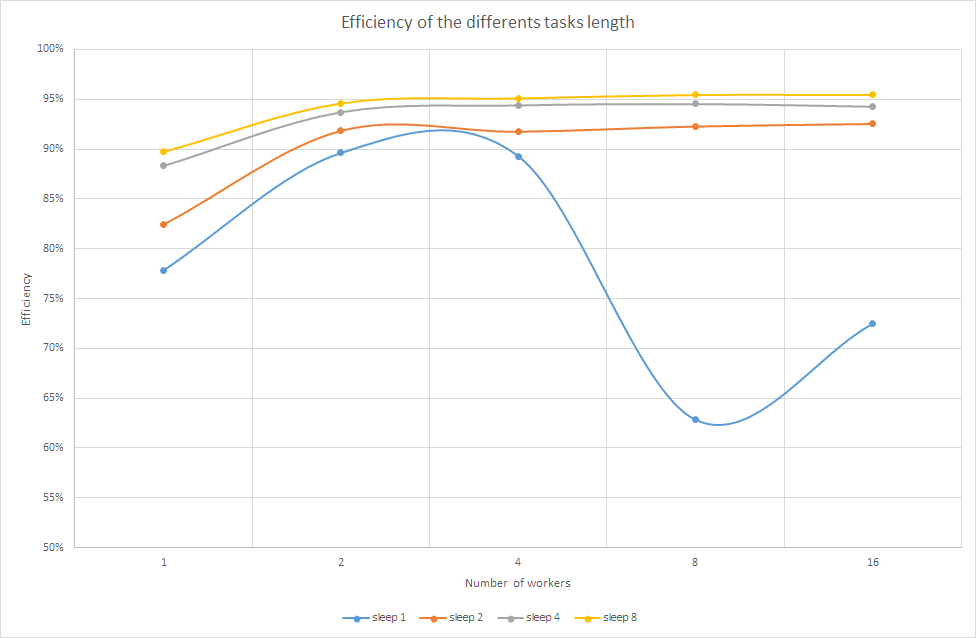
\includegraphics[width=0.9\textwidth]{efficiency_remote_workers.png}
\end{tabular}
\caption{Remote workers efficiency}
\end{figure}

For the remote workers, it seems obvious that the amount of workers and the nature of the worload might have consequences on the efficiency. We can observe that the efficiency increases and finally converge towards a 95\% efficiency limit for the 2, 4 and 8 seconds sleep workloads. However for the 1 second sleep, the system seems to not be scalable since we observe a drop of efficiency after running more than 4 workers. This may be due to the network induced delay which is longer compared to the task running time, but the fact that the curve goes back up for 16 workers is strange.

\subsection{Dynamic Provisioning}

In this part we will present the results of the latency evaluation and comparison between static and dynamic provisioning.\\
We did 5 measures of the time required to run a one-second sleep job on a single worker, which was either allocated statically or allocated dynamically by the provisioning module. On average, 63.6s are required for a static worker to do the aforementioned job, while 92.7s are required to detect the job, launch a worker, and run the job on it. We therefore mesured a 29.1s additional latency for the dynamic provisioning.\\
From that value we can assert that static provisioning is better suited for short execution job with a bursty arrival rate in queue, whereas the dynamic provisioning is better for longer execution time jobs or more regular job arrival rate since in the last 2 cases the latency is either irrelevant compared to the job length or the worker will not need to be shut down just after the job is done.

\section{Conclusion}
In this assignment we implemented a dynamic task provisioner, using SQS and DynamoDB, and added on top of this system a dynamic provisioning of workers. Our results show that our system is scalable for jobs of more than one second with an excellent efficiency. We have also noticed that for the kind of job we studied, we obtain a better thoughput for local workers than for remote workers. \\
Cloudwatch Amazon service could be an alternative to our implementation of dynamic provisioning.


\end{document}